\documentclass[10pt]{exam}

\usepackage{amssymb, amsmath, amsthm, mathrsfs, multicol, graphicx}
\usepackage{tikz}
\usetikzlibrary{calc}

\def\d{\displaystyle}
\def\?{\reflectbox{?}}
\def\b#1{\mathbf{#1}}
\def\f#1{\mathfrak #1}
\def\c#1{\mathcal #1}
\def\s#1{\mathscr #1}
\def\r#1{\mathrm{#1}}
\def\N{\mathbb N}
\def\Z{\mathbb Z}
\def\Q{\mathbb Q}
\def\R{\mathbb R}
\def\C{\mathbb C}
\def\F{\mathbb F}
\def\A{\mathbb A}
\def\X{\mathbb X}
\def\E{\mathbb E}
\def\O{\mathbb O}
\def\pow{\mathscr P}
\def\inv{^{-1}}
\def\nrml{\triangleleft}
\def\st{:}
\def\~{\widetilde}
\def\rem{\mathcal R}
\def\iff{\leftrightarrow}
\def\Iff{\Leftrightarrow}
\def\and{\wedge}
\def\And{\bigwedge}
\def\Vee{\bigvee}
\def\imp{\rightarrow}
\def\Imp{\Rightarrow}
\def\Fi{\Leftarrow}

\def\={\equiv}
\def\var{\mbox{var}}
\def\mod{\mbox{Mod}}
\def\Th{\mbox{Th}}
\def\sat{\mbox{Sat}}
\def\con{\mbox{Con}}
\def\bmodels{=\joinrel\mathrel|}
\def\iffmodels{\bmodels\models}
\def\dbland{\bigwedge \!\!\bigwedge}
\def\dom{\mbox{dom}}
\def\rng{\mbox{range}}
\DeclareMathOperator{\wgt}{wgt}

\def\circleA{(-.5,0) circle (1)}
\def\circleAlabel{(-1.5,.6) node[above]{$A$}}
\def\circleB{(.5,0) circle (1)}
\def\circleBlabel{(1.5,.6) node[above]{$B$}}
\def\circleC{(0,-1) circle (1)}
\def\circleClabel{(.5,-2) node[right]{$C$}}
\def\twosetbox{(-2,-1.5) rectangle (2,1.5)}
\def\threesetbox{(-2,-2.5) rectangle (2,1.5)}


\def\bar{\overline}

%\pointname{pts}
\pointsinmargin
\marginpointname{pts}
\marginbonuspointname{pts-bns}
\addpoints
\pagestyle{head}
\printanswers

\firstpageheader{Math 228}{\bf Homework 11 - Extra Credit}{Due: Friday, December 1}

\def\vertexsize{4 pt}
\newcommand{\vtx}[2]{node[fill,circle,inner sep=0 pt, minimum size=\vertexsize,label=#1:#2]{}}
\newcommand{\va}[1]{\vtx{above}{#1}}
\newcommand{\vb}[1]{\vtx{below}{#1}}
\newcommand{\vr}[1]{\vtx{right}{#1}}
\newcommand{\vl}[1]{\vtx{left}{#1}}
\renewcommand{\v}{\vtx{above}{}}

\begin{document}
\noindent \textbf{Instructions}: This is an extra homework assignment for those of you looking to boost your homework grade. There are \numquestions\, exercises that total \numpoints\, points. You do not have to complete the entire assignment to get credit. However, these problems are also a nice review for the final. Same rules as usual -- turn in your work on separate sheets of paper.  You must justify all your answers for full credit.

As usual, you are encouraged to work with classmates on the assignment, but make sure your final writeup is in your own words.  You are not permitted to use the Internet to search for answers.

\begin{questions}


%Replace with 3-part pie counting problem?  This is too easy.
% \question[6] Fifth grade students at a local elementary school took a poll about how they got to school. Many students took multiple modes of transportation with 31 students saying they got rides from their parents, 32 taking their bike to school and 21 walking. 8 students who said they bike also walk, and 3 students who usually walk get rides from their parents on some mornings. The one student that said he uses his bike and gets ride also said he uses all three modes of transportation.
% \begin{parts}
% \part Draw a Venn diagram of this situation.
% \begin{solution}
% 	\begin{center}
% 	\includegraphics[height=2 in, width=2 in]{venndiagramh12}
% 	\end{center}
% \end{solution}
% \part How many students took the survey?
% \begin{solution}
% 	Adding up all the values in the Venn diagram we get that there were 73 students who took the survey.
% \end{solution}
% \part How does this problem relate to PIE?
% \begin{solution}
% 	Remember that PIE is the principle of inclusion/exclusion and this problem relates because we want to calculate the total number of students who took the survey but we can't just add up all the numbers in the problem because we would be counting certain students multiple times. So, this means that when we are looking at this problem we need to follow the principle for 3 different sets which gives us: \[|A\cup B \cup C|=|A|+|B|+|C|-|A\cap B|-|A\cap C| - |B \cap C|+|A\cap B\cap C|\]
% So, we could have just looked at the problem and related each set of students to each $A, B, C$ where $A\cap B$ is the number of students who did both $A$ and $B$ to get to school.
% \end{solution}
% \end{parts}


\question[4] My circular kitchen table has 4 chairs (and we will assume the position of these chairs is important; one is facing away from the TV, for example).  Before our second kid, when we ate dinner, my wife and I sat across from each other and our daughter sat in the chair between us on my right (the chair to my left was empty).
\begin{parts}
  \part Occasionally, my daughter wanted us to sit in different chairs than usual.  For example, she would want to sit in my seat, want me to sit in my wife's seat, and my wife to sit in the chair that is usually empty.  How many different seating arrangements are possible?  Explain your answer carefully.
  \begin{solution}
    There are 4 chairs for my daughter to sit in, then 3 for my wife, and 2 for me.  So there are $4\cdot 3 \cdot 2 = 24$ seating arrangements.  Note this is simply $P(4,3)$.
  \end{solution}
  \part When she was feeling especially toddler-like, she would insist that none of us sit in our regular chairs.  How many of the seating arrangements you found in the previous part have this property?  Explain.
  \begin{solution}
    Let's say the normal arrangement of seats is ESMO (empty, Shannon, Maddie, Oscar).  It would not be too difficult to list all of the acceptable seating arrangements here.  In fact, we could list all 24, and cross out any that have one or more people in their usual seats.  Note that it is okay for E to be in the first spot, but S must be in a spot other than the second, M must be in spot other than the third, and O must be in a spot other than the 4th.  This is the list we would be left with:
    \[ EMOS, EOSM, SEOM, SOEM, SMOE, MEOS, MOES, MOSE, OESM, OMES, OMSE\]
    If you wanted to count this using our counting techniques, you could use PIE.  Count the number of \emph{unacceptable} arrangements and subtract that from 24:
    \[24-\left[3\cdot 2 + 3 \cdot 2 + 3 \cdot 2 - 2 - 2 - 2 + 1\right] = 11.\]
    Here each $3\cdot 2$ counts the number of ways that the other two people can sit if one person sits in their usual seat, the 2's count the number of choices for the last person when two people sit in their usual seat, and the 1 is the number of arrangements when all three people sit in their usual seat.
  \end{solution}
\end{parts}


\question[6] Consider bit strings.  Note that all the answers below should be easy to count directly by listing them, but you are asked to show how you can use the Principle of Inclusion/Exclusion to complete the problem.
\begin{parts}
  \part Use PIE to count the number of 5-bit strings of weight 4 that either start with 111 or end with 111 (or both).  Explain each part of your expression and why they are combined the way they are.
  \begin{solution}
    There are ${2 \choose 1}$ strings that start with 111 (two spots left, one of which must be a 1), ${2 \choose 1}$ strings that end with 111, and 0 strings that both start and end with 111.  Thus all together there are $2 + 2 - 0 = 4$ strings.
  \end{solution}
  \part Use PIE to count the number of 5-bit strings of weight 4 that contain 111 somewhere in them (which will be at the start, in the middle, at the end or more than one of these).
  \begin{solution}
    Start with 111: 2. Have 111 in the middle: 2.  End with 111: 2.  Start with 111 and have 111 in the middle: 1.  Have 111 in the middle and end with 111: 1.  Start and end with 111: 0.  All three: 0.  Thus
    \[2 + 2 + 2 - 1 -1 - 0 + 0 = 4\]
  \end{solution}
  \part Generalize PIE to 4 sets to count the number of 6-bit strings of weight 5 that contain 111 somewhere in them.
  \begin{solution}
    Consider the 4 positions the 111 string can occur: (a) first three bits, (b) second three bits, (c) third three bits, and (d) last three bits.  (a) can happen in ${3 \choose 2} = 3$ ways, as can (b), (c), and (d).  What about combinations of two?  (a) and (b): ${2 \choose 1}= 2$, (a) and (c): 1.  (a) and (d): 0.  (b) and (c): 2.  (b) and (d): 1.  (c) and (d): 2.  Combinations of 3?  (a), (b), and (c) can happen in 1 way, as can (b), (c), and (d), but the other two cannot happen.  Similarly, there is no way for all four to occur.  Putting this together gives:
    \[3 +3 +3+3 - 2 -1 - 0 -2 - 1 - 2 + 1+ 1 + 0 + 0 - 0 = 6.\]
    This makes sense since all of the 6 length-6-weight-5 bit strings contain 111 somewhere.
  \end{solution}
\end{parts}



%Have I already used this/is the answer in the book?  Answer in book, but with different numbers.  OK
\question[8] {\em Conic}, your favorite math themed fast food drive-in offers 18 flavors which can be added to your soda.  You have enough money to buy a large soda with 3 added flavors.  How many different soda concoctions can you order if:
\begin{parts}
  \part you refuse to use any of the flavors more than once?
  \part you refuse repeats but care about the order the flavors are added?
  \part you allow yourself multiple shots of the same flavor?
  \part you allow yourself multiple shots, and care about the order the flavors are added?
\end{parts}

  \begin{solution}
   \begin{parts}
    \part ${18 \choose 3}$ (order does not matter and repeats are not allowed)
    \part $P(18, 3) = 18\cdot 17\cdot 16$ (order matters and repeats are not allowed)
    \part ${20 \choose 17}$ (order does not matter and repeats are allowed: stars and bars)
    \part $18^3$ (order matters and repeats are allowed - 20 choices 4 times)
   \end{parts}
  \end{solution}


% %OK, although the solution could be cleaned up.
% \question[4] How many 10-digit numbers contain exactly four 1's, three 2's, two 3's and one 4?  Find the answer in two different ways to establish a binomial identity.
% \begin{solution}
%
% Some examples of acceptable outcomes: 1111222334, 1212121343, 4332221111, \ldots.  Each of these has 10 digits (as the questions states), and the number of each type of digit is the same.  It is just the arrangement that matters.  So does order matter here?  Maybe, but the order of what?  The digits?
%
% How could I break the task of choosing an outcome into subtasks?  One way would be to first select what goes in the first digit, then in the second, etc.  In this sense order does matter.  Does that work?  Well there are 4 choices for the first digit.  For the second digit there are... well it depends on what I choose for the first digit.  So this doesn't work.  Let's try something else.
%
% What if I first select where I put the 4.  It could go 1st, 2nd, etc.  There are 10 spots.  Thus 10, or maybe ${10 \choose 1}$.  Now where can I put the 3's.  It doesn't matter which 3 I place first, so here order does not matter.  I've already filled up one spot with a 4, so there are 9 spots left and I need 2 of them.  So ${9 \choose 2}$.  Ah, then ${7 \choose 3}$ to pick the three spots to put the 2's and ${4 \choose 4}$ choices of where to put the four 1's.  Now do I add or multiply?  Well to get my 10 digit number I need to do all these subtasks, not just one of them, so definitely multiply.  Thus the answer is
% \[{10 \choose 1}{9 \choose 2}{7 \choose 3}{4 \choose 4} = 12600\]
% Oh wait, what if I picked where the 1's went first?  There are ${10 \choose 4}$ spots, which leaves ${6 \choose 3}$ choices for where to put the 2's, and ${3 \choose 2}$ for the 3's and ${1 \choose 1}$ for the 4.  So now it looks like the answer should be
% \[{10 \choose 4}{6 \choose 3}{3 \choose 2}{1 \choose 1}\]
% Which is it?  Oh wait, those are the same.  Yay.
%
% Let me check one more thing.  Did I get everything?  Did I double count?  Maybe let's try building one of the outcomes using the answer (the first one).  The first thing I do is pick on of 10 things.  10 spots.  So for example, I could pick this:
% \[- - - - - ~ 4 - - - -\]
% Next I pick 2 out of 9 things.  Those 9 things are\ldots, the 9 remaining spots.  What do I do with the 2 that I pick?  I put in 3's.  So maybe:
% \[3 - - - - ~ 4 - 3 - -\]
% Yeah, and I was right to use ${9 \choose 2}$ instead of $P(9,2)$ because it does not matter if I pick the 1st spot and then the 8th, or the 8th and then the 1st.  Next I choose 3 out of 7\ldots spots to\ldots put 2's into.  Maybe I get
% \[3 - 2 2 - 4 - 3 - 2\]
% and then put the 1's in the remaining 4 spots - ${4 \choose 4} = 1$, and yes, there is just one way to finish up:
% \[3 1 22141312\]
% And that is an acceptable outcome.  Double yay.
% \end{solution}



\question[6] Consider the recurrence relation $a_n = 3a_{n-1} + 10a_{n-2}$.

\begin{parts}
  \part Find the general solution to the recurrence relation.  That is, find a closed formula for the $n$th term of the sequence, although this will have two parameters that would depend on initial conditions.
  \part If this recurrence relation described the number of $1\times n$ paths you can make using squares and dominoes in various colors, how many colors of each would you have?
	\part Using the context from part (b), give initial conditions and find the specific closed formula for the recurrence relation subject to the initial conditions.
\end{parts}
%FIX:
  \begin{solution}
  \begin{parts}
  \part $a_n = a(5)^n + b(-2)^n$, using the characteristic root technique.
  \part There must be 3 colors of squares and 10 colors of dominoes.
  \part The initial conditions would then be $a_1 = 3$ and $a_2 = 19$.  This gives a closed formula: $a_n = \frac{5}{7}(5)^n + \frac{4}{7}(-2)^n$.
  \end{parts}
  \end{solution}





\question[6] Consider the binomial identity $\d {3 \choose 0} + {4 \choose 1} + {5 \choose 2} + \cdots + {3+n\choose n} = {4+n \choose n}$.  It might be helpful to ``find'' this in Pascal's Triangle.
\begin{parts}
	\part Prove the identity using a combinatorial proof.  Hint: if you think about $n$-topping pizzas, which topping could be the ``last''?
	\part Prove the identity using mathematical induction.  Hint: you know a recurrence relation for the binomial coefficients---look at Pascal's Triangle.
\end{parts}


\begin{solution}
  \begin{parts}
    \part Consider the counting question: how many $n$-topping pizzas can you create if you have $n+4$ toppings?   One answer is clearly ${4+n \choose n}$.  Alternatively, you could break this up into cases by which topping is alphabetically the first one you don't choose.  If this is the 4th on your alphabetical list of toppings, then you picked 0 of the first three (and all the remaining $n$).  If this one is 5th on the list, then of the first 4, you must pick 1 (plus the remaining $n-1$).  If the last one is the 6th on the list, there are $n-2$ toppings you must choose, but of the first 5, you must choose 2.  And so on.  If you don't choose the last topping, then of the first $n+3$ you choose $n$.
    \part Let $P(n)$ be the statement, $\d {3 \choose 0} + {4 \choose 1} + {5 \choose 2} + \cdots + {3+n\choose n} = {4+n \choose n}$.

    Base case: ${3 \choose 0} = 1 = {4 \choose 0}$ when $n = 0$.

    Inductive case.  Assume $P(k)$ is true.  Now
    \[\d {3 \choose 0} + {4 \choose 1} + {5 \choose 2} + \cdots + {3+k\choose k} = {4+k \choose k}\]
    so,
    \[\d {3 \choose 0} + {4 \choose 1} + {5 \choose 2} + \cdots + {3+k\choose k} + {3+k+1 \choose k+1} = {4+k \choose k} + {3+k+1 \choose k+1}\]
    but the left hand side is the same as $\d {4 + k+1 \choose k+1}$ by the recurrence relation ${n\choose k} = {n-1 \choose k-1} + {n-1 \choose k}$ (each entry in Pascal's triangle is the sum of the two entries above it).  Thus $P(k+1)$ is true.

    Therefore, by the Principle of Mathematical Induction, $P(n)$ is true for all $n \ge 0$
  \end{parts}
\end{solution}


% % What about the new Hamilton path exercise from the book?
% \question[6] We say that a graph has a {\em Hamilton path} if there is a path which visits each vertex exactly once (you do not need to use every edge in the path).
% \begin{parts}
%   \part Suppose a graph has a Hamilton path.  What is the maximum number of vertices of degree one the graph can have?  Explain why your answer is correct.
%
%   \begin{solution}
%     Note that a vertex of degree one can only be the start or the end of a Hamilton path - if we go {\em to} a vertex of degree one, we are stuck there - we cannot use the same edge to leave the vertex, because doing so would bring us back to a vertex we have already visited.  If a graph has a Hamilton path, it might start at a vertex of degree one, end at a vertex of degree one, but there cannot be any other vertices of degree one.  Therefore a graph with a Hamilton path can have at most two vertices of degree one.
%   \end{solution}
%
%   \part Find a graph which does not have a Hamilton path even though no vertex has degree one.  Explain why your example works.
%
%   \begin{solution}
%     There are many such graphs.  Here are two examples:
%
%     \begin{center}
%       \begin{tikzpicture}
%         \draw[thick] (-1,0) \v -- (0,1) \v -- (1, 0) \v -- (0, .33) \v -- (-1,0) -- (0,-.33) \v -- (1,0) -- (0,-1) \v -- (-1,0);
%       \end{tikzpicture}
%       \hspace{1in}
%       \begin{tikzpicture}
%         \draw[thick] (270:.5) \v -- (255:1) \v -- (285:1) \v -- (270:.5) -- (0,0) \v -- (135:.5) \v -- (150:1) \v -- (120:1) \v -- (135:.5) (0,0) -- (45:.5) \v -- (60:1) \v -- (30:1) \v -- (45:.5);
%       \end{tikzpicture}
%
%     \end{center}
%
%   \end{solution}
%
% \end{parts}

%Good:
\clearpage
\question[4] Can you distribute conjunctions over disjunctions?  Disjunctions over conjunctions?  Let's find out.  Remember, two statements are logically equivalent if they are true in exactly the same cases.
\begin{parts}
  \part Are the statements $P \vee (Q \and R)$ and $(P \vee Q) \and (P \vee R)$ logically equivalent?
  \begin{solution}
    Yes they are.  We prove this by showing that their truth tables are identical:
    \begin{center}
        \begin{tabular}{c|c|c||c||c}
    $P$ & $Q$ & $R$ & $P \vee (Q \and R)$ & $(P \vee Q) \and (P \vee R)$\\ \hline
    T & T & T & T & T\\
    T & T & F & T & T \\
    T & F & T & T & T \\
    T & F & F & T & T \\
    F & T & T & T & T \\
    F & T & F & F & F \\
    F & F & T & F & F \\
    F & F & F & F & F
  \end{tabular}
    \end{center}
  \end{solution}

  \part Are the statements $P \and (Q \vee R)$ and $(P \and Q) \vee (P \and R)$ logically equivalent?
  \begin{solution}
    It works again.  Here are the two truth tables which prove it:
        \begin{center}
        \begin{tabular}{c|c|c||c||c}
    $P$ & $Q$ & $R$ & $P \and (Q \vee R)$ & $(P \and Q) \vee (P \and R)$\\ \hline
    T & T & T & T & T\\
    T & T & F & T & T \\
    T & F & T & T & T \\
    T & F & F & F & F \\
    F & T & T & F & F \\
    F & T & F & F & F \\
    F & F & T & F & F \\
    F & F & F & F & F
  \end{tabular}
    \end{center}
  \end{solution}

\end{parts}


%OK
\question[4] While walking through a fictional forest, you stumble upon two trolls playing Stratego\textsuperscript{\textregistered}.  As you are well aware, all trolls are either knights who always tell the truth or knaves who always lie.  These two trolls tell you:
\begin{itemize}
\item[]Troll 1: If we are cousins, then we are both knaves.
\item[]Troll 2: We are cousins or we are both knaves.
\end{itemize}
 Could both trolls be knights?  Prove your answer.  Your explanation should pay careful attention to the logical form of the statements, and perhaps even use truth tables.

\begin{solution}
This is relatively easy to sort out if you use truth tables.  Let $P$ be ``We are cousins,'' and $Q$ be ``We are both knaves.''  We then get the truth table describing the statements:

\centerline{
\begin{tabular}{c|c|c|c}
$P$ & $Q$ & $P \imp Q$ & $P \vee Q$ \\ \hline
T & T & T & T\\
T & F & F & T \\
F & T & T & T \\
F & F & T & F
\end{tabular}
}

Note that right away you can see that it is impossible for both trolls to be \emph{knaves}, since there is no case in which both of their statements are false.  From this we can conclude that the statement $Q$ is false!  So we are in rows 2 or 4.  But in each of these, one or the other troll is lying, so it is impossible for both to be knights.
\end{solution}









\question[6] Recall that a Hamilton path is a walk that visits every vertex exactly once.  A Hamilton cycle is is a Hamilton path that starts and stops at the same vertex (it is okay that the starting/stopping vertex is visited twice, but no other vertex may be).  Consider the following graph:

\begin{center}
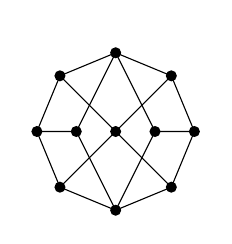
\begin{tikzpicture}[scale=.5]
\foreach \x in {0, 45, ..., 315}
  \draw  (\x:2) \v -- (\x+45:2);
\draw (0,0) \v -- (45:2) (0,0) -- (135:2) (0,0) -- (225:2) (0,0) -- (315:2);
\draw (-1,0) \v -- (90:2) (-1,0) -- (180:2) (-1,0) -- (270:2);
\draw (1,0) \v -- (90:2) (1,0) -- (0:2) (1,0) -- (270:2);
\end{tikzpicture}
\end{center}

\begin{parts}
	\part Find a Hamilton path.  Can your path be extended to a Hamilton cycle?
	\part Is the graph bipartite?  If so, how many vertices are in each ``part''?
	\part Use your answer to part (b) to prove that the graph has no Hamilton cycle.  What can you say in general about bipartite graphs and Hamilton cycles?
\end{parts}

\begin{solution}
  \begin{parts}
    \part One path is shown below:

    \begin{center}
    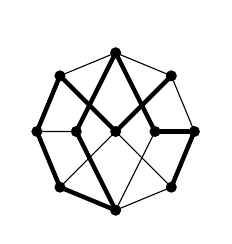
\begin{tikzpicture}[scale=.5]
    \foreach \x in {0, 45, ..., 315}
      \draw  (\x:2) \v -- (\x+45:2);
    \draw (0,0) \v -- (45:2) (0,0) -- (135:2) (0,0) -- (225:2) (0,0) -- (315:2);
    \draw (-1,0) \v -- (90:2) (-1,0) -- (180:2) (-1,0) -- (270:2);
    \draw (1,0) \v -- (90:2) (1,0) -- (0:2) (1,0) -- (270:2);
    \draw[ultra thick] (45:2) -- (0,0);
    \draw[ultra thick] (0,0) -- (135:2);
    \draw[ultra thick] (135:2) -- (180:2);
    \draw[ultra thick] (180:2) -- (225:2);
    \draw[ultra thick] (225:2) -- (270:2);
    \draw[ultra thick] (270:2) -- (-1,0);
    \draw[ultra thick] (-1,0) -- (0,2);
    \draw[ultra thick] (0,2) -- (1,0);
    \draw[ultra thick] (1,0) -- (2,0);
    \draw[ultra thick] (2,0) -- (315:2);
    \end{tikzpicture}
    \end{center}
    This path cannot be extended to a cycle (none could be, as seen below).
    \part Yes, the graph is bipartite. In other words you could 2-color the vertices.  Notice that doing so always gives one side/color 5 vertices and the other 6.
    \part Notice that any Hamilton path (or cycle) must alternate between sides/colors of the bipartite graph.  To have a path, we must start at one of the vertices on the larger side, but then after visiting all 11 vertices, we will be back on the larger side, so we will not be able to travel to the starting vertex (which is a different vertex on the same side).  In general, this says that if a bipartite graph has a Hamilton cycle, then the two sides of the bipartite graph must have the same size.
  \end{parts}
\end{solution}




%\question[6] Develop your own story problem for a graph that has an Euler path. Your problem must have at least two parts.
%%\begin{solution}
%%
%%\end{solution}

% \question[4] Prove that every graph has an even number of vertices that have odd degree.  Say what style of proof you are using (direct, contrapositive, contradiction, induction, or combinatorial)
% \begin{solution}
% 	We will give a proof by contradiction.
%
% 	Suppose for a contradiction that there exists a graph that has an odd number of vertices with odd degree. Then, if we added up all the degrees of each vertices, we could get an odd number because an odd plus an odd an odd number of times is odd. Now, this creates an issue when we go to calculate the number of edges of the graph by dividing the total number of degrees by 2 because we will get half of an edge, which is not possible. Therefore, every graph that contains vertices of an odd degree must contain an even number of them.
% \end{solution}









\question[6] Suppose $G$ is a graph with 7 vertices.  Consider the statement:

\centerline{\textit{If $G$ has an Euler circuit, then there are at least 3 vertices with the same degree.}}

\begin{parts}
\part Write the \underline{first line} of a proof of the statement using each specified style of proof:

Direct proof:
\begin{solution}
Assume $G$ has an Euler circuit.
\end{solution}
Proof by contrapositive:
\begin{solution}
Assume there are at most 2 vertices with the same degree. (Assume it is not the case that at least 3 vertices have the same degree.)
\end{solution}
Proof by contradiction:
\begin{solution}
Assume $G$ has an Euler circuit but there are at most 2 vertices with the same degree.
\end{solution}
\part  Prove the statement using an appropriate style of proof.  Hint: what could the degrees be?
\begin{solution}
\begin{proof}
Proceed by contradiction.  Assume $G$ has an Euler circuit and that there are at most 2 vertices sharing the same degree.  Since $G$ has an Euler circuit, every vertex has \emph{even} degree.  Thus the possible degrees are 2, 4, and 6 (you cannot have larger degree since there are only 7 vertices).  Since there are at most 2 vertices sharing the same degree, there are at most 6 vertices.  This contradicts the assumption that $G$ has 7 vertices.
\end{proof}
\end{solution}
\end{parts}





\question[5] In any graph, an \emph{independent set} is a subset of the vertices that are not adjacent to each other.  In other words, they are a set of vertices that could be colored the same in a proper vertex coloring.  Note that the empty set of vertices is independent  How many different independent sets are there in $P_{10}$, the path of 10 vertices (9 edges)?  Hint: this is intended to be a question about sequences.  You should give a recursive definition for the number of independent sets in $P_n$ and explain why it is correct.

\begin{solution}
Start with $P_2$ (a pair of adjacent vertices).  There are exactly 3 independent sets: the empty set and the two sets that contain just one vertex.  Now for $P_3$, think of adding in 1 vertex to the end of $P_2$.  We could put this new vertex in the independent set or not.  If we keep it out, then each independent set we had before is still independent (so that is 3 already).  If we put it in, then we only have 2 choices: put the vertex on the other end in or not.  Thus there are a total of 5 independent sets.

Now the fun begins.  Add a 4th vertex on the end of the path to get $P_4$.  If we keep this vertex out, we could use any of the 5 independent sets of $P_3$.  If we put it in, then we cannot put the vertex next to it in, so we just need to get an independent set on the remaining two vertices.  But that looks just like $P_2$, and we know there are 3 independent sets.  So we have $8$ independent sets in $P_5$.

It's the Fibonacci recurrence.  The number of independent sets in $P_n$ is the number in $P_{n-1}$ (if we keep the new vertex out) plus the number in $P_{n-2}$ (if we put the new vertex in).  Following this up to $P_{10}$ we see there will be 144 independent sets.
\end{solution}



\question[5] Use your knowledge of sequences and graph theory to find the number of edges, vertices and triangular faces (all but the outside) of the $n$th figure in the sequence started below.  For example, the 1st figure has $e = 12$, $v = 7$, and $f = 6$.

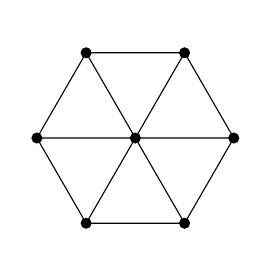
\begin{tikzpicture}[scale=1.25]
  \draw (0:0) \v;
  \foreach \x in {0,...,5}{
  \draw (0:0) -- (60*\x:1) \v -- (60*\x + 60: 1);
  }
\end{tikzpicture}
\hfill
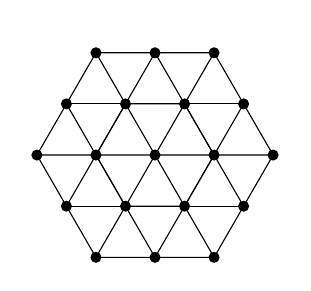
\begin{tikzpicture}[scale=.75]
  \draw (0:0) \v;
  \foreach \x in {0,...,5}{
  \draw (0:0) -- (60*\x:1) \v -- (60*\x + 60: 1) ;
  \draw (60*\x:1) -- (60*\x:2) \v -- (60*\x + 60:2);
  \draw ($ (60*\x:2)!.5!(60*\x + 60:2) $) \v -- ($ (60*\x+180:2)!.5!(60*\x + 120:2) $);
  }
\end{tikzpicture}
\hfill
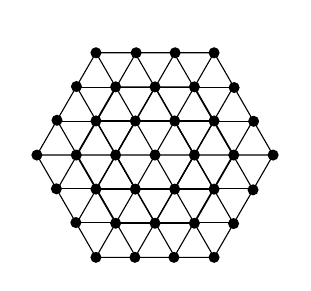
\begin{tikzpicture}[scale=.5]
  \draw (0:0) \v;
  \foreach \x in {0,...,5}{
  \draw (0:0) -- (60*\x:1) \v -- (60*\x + 60: 1) ;
  \draw (60*\x:1) -- (60*\x:2) \v -- (60*\x + 60:2);
  \draw ($ (60*\x:2)!.5!(60*\x + 60:2) $) \v -- ($ (60*\x+180:2)!.5!(60*\x + 120:2) $);
  \draw (60*\x:2) -- (60*\x:3) \v -- (60*\x + 60:3);
  \draw ($ (60*\x:3)!.33!(60*\x + 60:3) $) \v -- ($ (60*\x+180:3)!.33!(60*\x + 120:3) $);
    \draw ($ (60*\x:3)!.66!(60*\x + 60:3) $) \v -- ($ (60*\x+180:3)!.66!(60*\x + 120:3) $);
  }
\end{tikzpicture}
\hfill
$\cdots$

\begin{solution}
  First, we find the number of vertices in the $n$th figure to be $v_n = 3n^2 +3n + 1$ (you can use polynomial fitting, or notice that every time you add a larger multiple of 6 and use triangular numbers).

  Of these vertices, there will be 6 with degree 2 (the corners), $6n-6$ with degree 4 (the sides) and the rest, $3n^2 - 3n$ with degree 6.  Adding up the degrees and dividing by 2 gives the number of edges: $e_n = 9n^2 + 3n$.

  Finally, we can use Euler's formula to find the number of triangles.  However, since we don't want to count the outside, we would have
  \[f_n = 1 + 9n^2 + 3n - (3n^2 + 3n + 1) = 6n^2.\]
\end{solution}


% % Could be left off:
% \question[4] An inventory list consists of 115 items, each on its own numbered line, each marked ``available'' or ``unavailable.'' There are 60 items marked available. Show that there are at least two available items in the list exactly four lines apart.
% \begin{solution}
% 	Assume for a contradiction that there are no items marked available exactly 4 items apart. To do this, let us consider two different sets. The first set will be the number of available items: \[a_1,a_2,...,a_60\] and the second set will be the number of items that cannot be marked as available \[a_1+4,a_2+4,...a_{60}+4\]. Now, each of these sets has exactly 60 items and must be separate items on the overall list. However, there are only 115 items on the list, which means that at least 2 items from each set must be the same item. Therefore, there must be at least two available items in the list exactly four items apart.
% \end{solution}



%Mouse house?
%Converse/Contrapositive/Negation?








% \bonusquestion[4] {\bf BONUS:} Clu D. Tector was lecturing on methods for detecting counterfeit coins. To illustrate a point he removed four coins from his pocket, one of which is either heavier or lighter than the rest (in other words, it was counterfeit). He then pulled a fifth coin from his pocket and said it was a ``good'' coin. Next produced a balance scale and challenged the audience to suggest a plan for determining, in the fewest possible weighings, which of the four original coins was the counterfeit. He claimed you could do it in no more than two weighings. Describe how you would have to weigh the coins such that you would only have to only weigh the coins twice.
% \begin{solution}
% 	First, let's label each of the coins. The first four will be $A,B,C,D$ while the good coin will be $G$. Let's first measure $A,B$ against $C, G$. If the scale is balanced then we got lucky and $D$ is the counterfeit coin. Next, weigh $D$ against $G$ to figure out if it is heavy or light. However, it may be the case that that $A+B > C+G$ or $A+B < C+G$. If the first case is true then $D$ is a good coin, and either $C$ is light or $B$ or $A$ is heavy. Thus, a second weighting of $B$ against $A$ tells which coin is counterfeit. If $A=B$ then $C$ was the counterfeit and was lighter and if $A \not=B$ then whichever one weighed more is the counterfeit and is heavier. Similarly for $A+B<C+G$. In this case, either $C$ is heavy or $A$ or $B$ is light. Weigh $A$ against $B$ and if they are equivalent then $C$ is heavy. If not, then whichever one weighs less is the counterfeit and is lighter than the rest.
% \end{solution}
\end{questions}




\end{document}
